\chapter{Wprowadzenie}
\label{sec:chapter2}

\section{Aplikacja Ebook-Wizard}
\label{sec:ą:chapter2}
Aplikacja Ebook-Wizard została udostępniona w Internecie pod adresem \textit{\href{https://ebookwizard.danielrogowski.net}{https://ebookwizard.danielrogowski.net}}.

Serwis Ebook-Wizard został podzielony na dwa osobno uruchamiane procesy: serwer backend napisany w języku Java przy użyciu frameworka Spring oraz klient frontend napisany w języku TypeScript przy użyciu frameworka Angular. Oba komponenty komunikują się ze sobą za pośrednictwem protokołu HTTPS. Rozdział warstwy obliczeniowej (backend) oraz warstwy prezentacji (frontend) pozwolił na niezależny rozwój obu komponentów oraz na lepsze dopasowanie technologii do specyficznych zadań każdej z warstw. Pełny opis sposobu komunikacji frontendu z backendem, wraz z uzasadnieniem wyboru narzędzi, został szczegółowo omówiony w Rozdziale \ref{chapter:implementation}.

\section{Projekt funkcjonalności serwisu}

W procesie projektowania serwisu Ebook-Wizard zostały wydzielone dwa rodzaje zasobu: \textbf{plik e-booka} oraz \textbf{projekt e-booka}. Plik to pojedyncza książka zaimportowana przez użytkownika z dysku twardego. Jeden plik może występować w kilku wersjach (np. wersji pdf, docx, html), a więc do jednego pliku logicznego zdefiniowanego w bazie Ebook-Wizard dołączone może kilka plików fizycznych.

Projektem jest natomiast e-book, który został przez użytkownika utworzony od zera, i wypełniony treścią przy użyciu graficznego edytora projektu. Projekty i pliki są w Ebook-Wizard rozpatrywane jako dwa oddzielne zasoby, różniące się sposobem wyświetlania w interfejsie graficznym oraz sposobem implementacji ich obsługi.

Poniższa lista prezentuje pełną listę funkcjonalności, które zawiera aplikacja Ebook-Wizard.

\begin{enumerate}
    \item Operacje na plikach:
    \begin{enumerate}
        \item importowanie pliku z dysku twardego użytkownika,
        \item wyświetlanie listy plików użytkownika,
        \item sortowanie i przeszukiwanie listy plików,
        \item wyświetlanie metadanych i obrazu okładki pojedynczego pliku,
        \item zmiana metadanych i obrazu okładki książki,
        \item usuwanie pliku,
        \item przesyłanie pliku na fizyczny czytnik e-booków przez protokół e-mail,
        \item udostępnianie pliku w Internecie przez wygenerowanie hiperłącza,
        \item konwersja pliku do wybranego formatu,
        \item konwersja pliku na projekt,
        \item pobieranie pliku z serwisu na dysk twardy użytkownika,
        \item organizowanie plików w foldery,
        \item wyświetlanie treści pliku w interaktywnym czytniku online,
        \item dodawanie i usuwanie zakładek na stronach książki, 
        \item automatyczne generowanie audiobooka przez usługę syntezy głosu.
    \end{enumerate}
    
    \item Operacje na projektach:
    \begin{enumerate}
        \item tworzenie projektu,
        \item wyświetlanie listy projektów użytkownika,
        \item sortowanie i przeszukiwanie listy projektów,
        \item wyświetlanie szczegółów metadanych i obrazu okładki pojedynczego projektu,
        \item zmiana metadanych i obrazu okładki książki,
        \item usuwanie projektu,
        \item przesyłanie projektu na fizyczny czytnik e-booków,
        \item udostępnianie projektu w Internecie przez wygenerowanie hiperłącza,
        \item eksportowanie projektu do wybranego formatu,
        \item pobieranie wyeksportowanego projektu na dysk użytkownika,
        \item konwersja projektu na plik,
        \item edycja rozdziałów (dodawanie, usuwanie, zmienianie treści i kolejności rozdziałów).
        \item formatowanie ciała rozdziału (tworzenie list numerowanych i punktowanych, definiowanie wcięć, pogrubienie tekstu, pochylenie, podkreślenie, przekreślenie, zmiana czcionki, wyrównanie tekstu, definiowanie nagłówków, usuwanie formatowania)
        \item dodawanie i usuwanie ilustracji w ciele rozdziału
    \end{enumerate}
    
    \item Operacje użytkownika:
        \begin{enumerate}
        \item logowanie,
        \item rejestracja,
        \item resetowanie hasła,
        \item zmiana hasła, e-maila lub pseudonimu,
        \item zamykanie konta.
    \end{enumerate}

    \item Inne operacje i wymagania:
    \begin{enumerate}
        \item wyświetlanie limitu przestrzeni dyskowej użytkownika (dla każdego konta wynosi 500 MB),
        \item odrzucanie zapytań użytkownika, jeśli ich wykonanie przekroczyłoby limit dyskowy,
        \item odrzucanie plików większych niż 25 MB w celu ograniczenia obciążenia serwera,
        \item wyświetlanie regulaminu serwisu,
        \item wyświetlanie statystyk serwisu.
    \end{enumerate}
\end{enumerate}

\section{Wykaz wspieranych rozszerzeń}

W procesie projektowania aplikacji Ebook-Wizard wyszczególniono 7 formatów plików, które są obsługiwane przez aplikację. Wspomniane formaty to: epub, mobi, azw3, docx, txt, html, pdf. Przy użyciu aplikacji Ebook-Wizard użytkownik może zaimportować z dysku dowolny plik o wspieranym formacie, i przekonwertować go na inny wspierany format.

Wymienione rozszerzenia można podzielić na dwa rodzaje: formaty ogólnego użytku oraz formaty dedykowane czytnikom e-booków. Formaty dedykowane czytnikom gwarantują poprawne wyświetlanie e-booka na dedykowanym czytniku e-booków. Pliki opracowane w tych formatach zawierają osadzone metadane, dzięki którym czytnik jest w stanie wyświetlić informacje takie jak imię i nazwisko autora, tytuł książki, czy obraz okładki.

Formaty dedykowane czytnikom nie zawierają informacji na temat podziału na strony (w przeciwieństwie na przykład do formatu pdf), dzięki czemu e-book może się skalować i wyświetlać poprawnie na urządzeniu o dowolnym rozmiarze. \cite{format_comparision}

Formaty pdf, docx, txt oraz html są formatami ogólnego użytku, niedostosowanymi do wyświetlania na czytnikach. Mimo to, aplikacja Ebook-Wizard wspiera te formaty, gdyż niektórzy użytkownicy mogą preferować korzystanie z tego typu formatów.

W Tabeli \ref{tab:ebook_wizard_formats} przedstawiono porównanie formatów obsługiwanych przez aplikację Ebook-Wizard.

\begin{table}
    \renewcommand{\arraystretch}{1.5} % Ustawienie minimalnej wysokości rzędu
    \caption{Przedstawienie formatów plików obsługiwanych przez Ebook-Wizard}

    \centering
    \begin{tabular}{|>{\centering\arraybackslash}c|>{\centering\arraybackslash}c|>{\centering\arraybackslash}m{2cm}|>{\raggedright\arraybackslash}m{5.5cm}|>{\centering\arraybackslash}m{2cm}|>{\centering\arraybackslash}m{2cm}|}
        \hline
        Lp. & Nazwa & Rozwinięcie  & Opis  & Dedykowany czytnikom? & Wspiera osadzanie obrazów? \\
        \hline
        1   & MOBI  & Mobipocket & Format e-book stworzony przez firmę Mobipocket. Używany głównie przez urządzenia Kindle przed wprowadzeniem AZW3. & Tak & Tak \\
        \hline
        2   & PDF  & Portable Document Format & Format dokumentu opracowany przez Adobe, szeroko stosowany do przechowywania dokumentów tekstowych oraz grafiki. & Nie & Tak \\
        \hline
        3   & AZW3  & \textit{Nieznane} & Nowsza wersja formatu MOBI, używana przez urządzenia Kindle. Obsługuje bardziej zaawansowane opcje formatowania i osadzania multimediów. & Tak & Tak \\
        \hline
        4   & DOCX  & Document XML & Format plików Microsoft Word oparty na standardzie XML. & Nie & Tak \\
        \hline
        5   & TXT  & Plain Text & Format tekstowy, który nie zawiera żadnych informacji o formatowaniu. & Nie & Nie \\
        \hline
        6   & HTML  & Hypertext Markup Language & Standardowy format dla stron internetowych. Może zawierać tekst, obrazy, linki i inne elementy. & Nie & Tak \\ \hline
        7   & EPUB  & Electronic Publication & Archiwum zip zawierające pliki html z treścią publikacji, pliki ilustracji oraz plik XML z metadanymi. & Tak & Tak \\
        \hline
    \end{tabular}
    \label{tab:ebook_wizard_formats}
\end{table}

\section{Wykaz wspieranych metadanych}

Ebook-Wizard wspiera konfigurację następujących metadanych przechowywanych e-booków: tytuł książki, autor, opis, lista tagów, obraz okładki. 

Pełne możliwości osadzania metadanych mają wyłącznie formaty dedykowane czytnikom, czyli epub, mobi oraz azw3. \cite{format_comparision} W przypadku innych formatów, te możliwości są ograniczone (np. format txt nie ma możliwości osadzenia jakichkolwiek metadanych). Jeśli dany format nie wspiera osadzania metadanych, metadane są wyświetlane wyłącznie w graficznym interfejsie Ebook-Wizard. Jeśli dany format pliku umożliwia osadzania metadanych, wówczas Ebook-Wizard zmodyfikuje plik i opatrzy go podanymi przez użytkownika metadanymi. Producenci czytników e-booków często korzystają z tych metadanych, aby zamiast nazwy pliku wyświetlać na czytniku faktyczną nazwę książki i skonfigurowany obraz okładki.

\section{Przegląd istniejących rozwiązań}

\subsection{Aplikacja Calibre}
Calibre jest jedną z najpopularniejszych aplikacji do zarządzania zbiorem e-booków. Według statystyk umieszczonych na stronie projektu Calibre, w dniu 19.11.2024 r. aplikacja miała 2.807.669 aktywnych użytkowników. \cite{calibre_usage_statistics}

Calibre jest aplikacją z interfejsem graficznym, która dostępna jest na systemy operacyjne: Windows, macOS oraz Linux. Jest to projekt oparty na licencji GNU GPL 3.0 \cite{calibre_user_manual}, co oznacza, że za korzystanie z Calibre nie jest pobierana żadna opłata. \cite{gpl}

Głównymi funkcjami oferowanymi przez program Calibre jest gromadzenie e-booków, konwertowanie ich pomiędzy wspieranymi formatami oraz modyfikacja metadanych osadzonych w pliku (np. zmiana nazwy, opisu, obrazu okładki). \cite{calibre_user_manual}

\begin{figure}[h]
    \centering
    \setlength{\fboxsep}{0pt}
    \setlength{\fboxrule}{0.4pt}
    \fbox{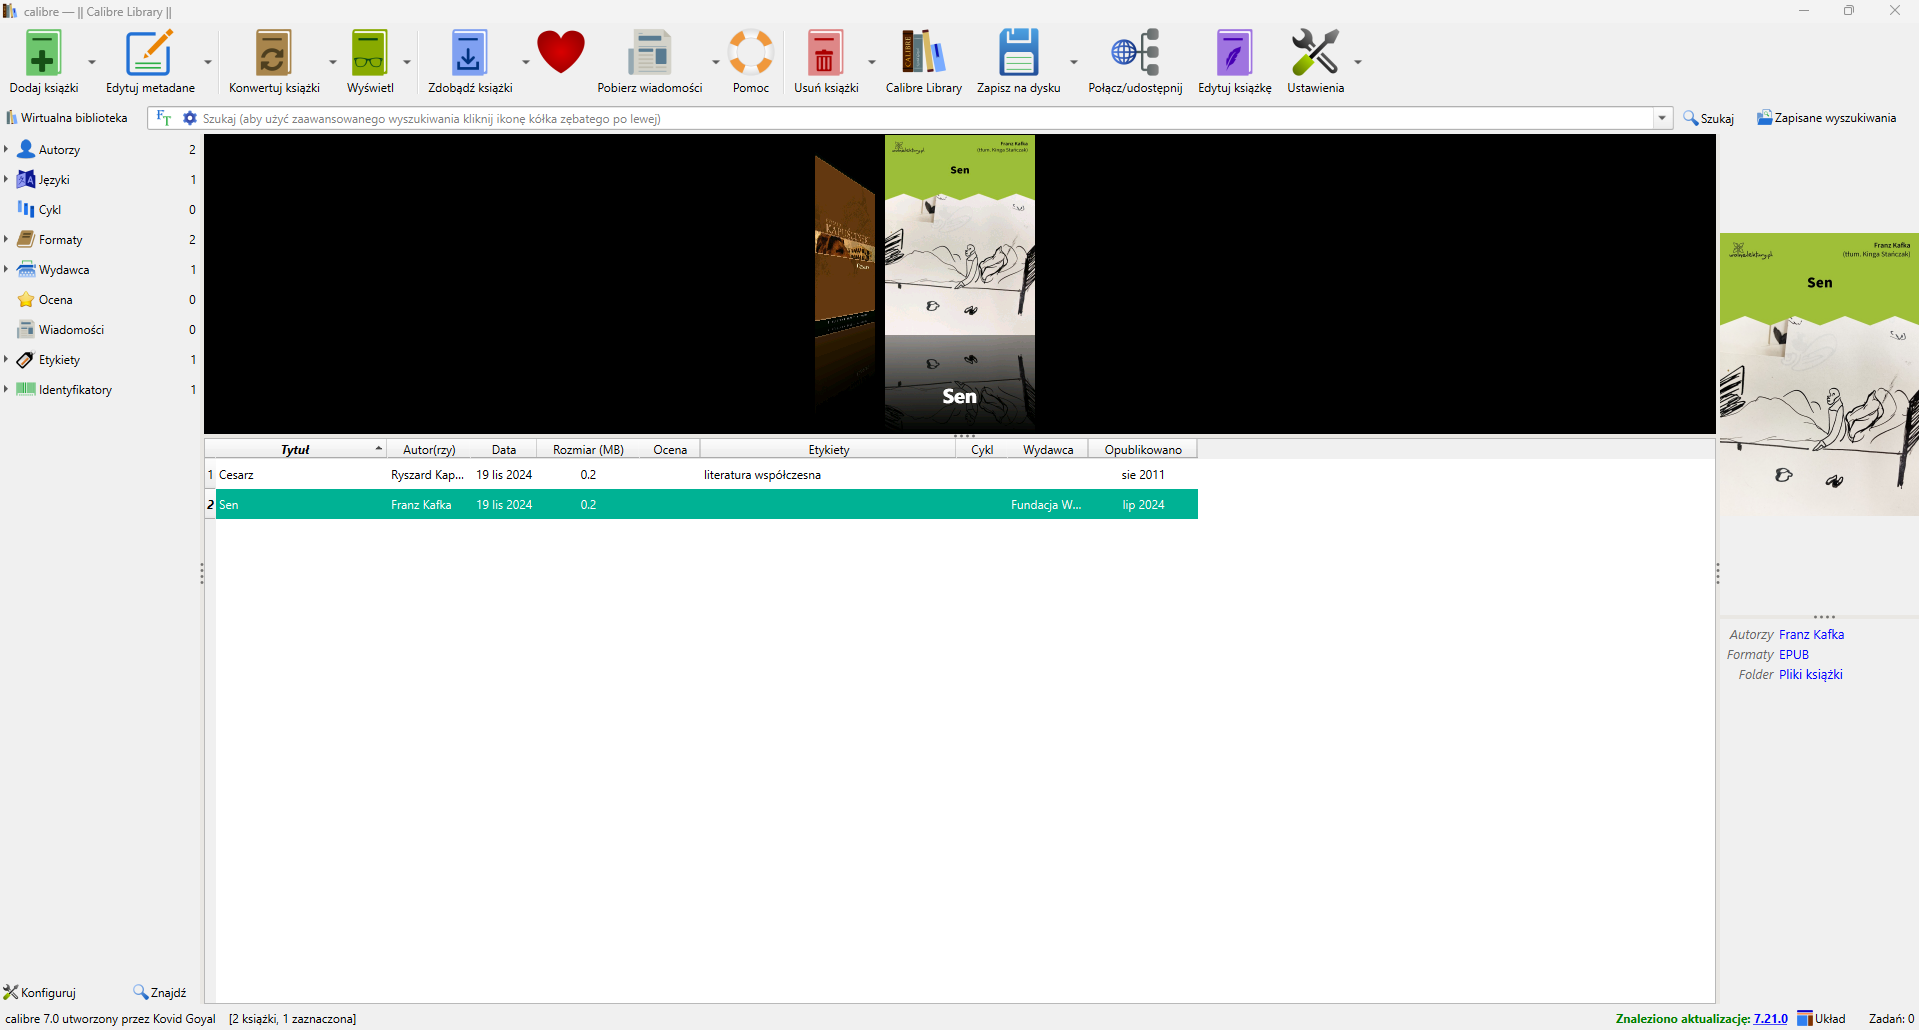
\includegraphics[width=0.9\textwidth]{chap2/calibre_interface.png}}
    \caption{Interfejs graficzny programu Calibre}
    \label{fig:obrazek_z_ramką}
\end{figure}

Calibre wspiera możliwość przesłania e-booka z programu na fizyczny czytnik na dwa sposoby: poprzez przesłanie go protokołem e-mailowym na adres nasłuchiwany przez urządzenie, lub bezpośrednio przez podłączenie czytnika kablem USB do komputera. Z racji na swoje środowisko uruchomieniowe (przeglądarka internetowa), Ebook-Wizard nie wspiera bezpośredniego podłączenia czytnika kablem. Przewagą Ebook-Wizarda jest natomiast to, że nie wymaga konfigurowania protokołu e-mailowego. Calibre wymaga dostarczenia loginu i hasła do własnego konta pocztowego, natomiast Ebook-Wizard korzysta z globalnej usługi wysyłania e-maili, dostarczanej przez serwer backendowy.

Calibre posiada szczątkowe wsparcie dla edytowania treści e-booka, jednakże polega ono na ręcznej modyfikacji kodu HTML oraz CSS książki. Ebook-Wizard oferuje graficzny edytor WYSIWYG\footnote{WYSIWYG (ang. \textit{What You See Is What You Get}) - forma edytora, który wyświetla edytowany dokument w sposób wizualny; przykładem edytora WYSIWYG jest program Microsoft Word.} dzięki czemu może być używany również przez użytkowników nie mających doświadczenia ze wspomnianymi językami.

\begin{figure}[h]
    \centering
    \setlength{\fboxsep}{0pt}
    \setlength{\fboxrule}{0.4pt}
    \fbox{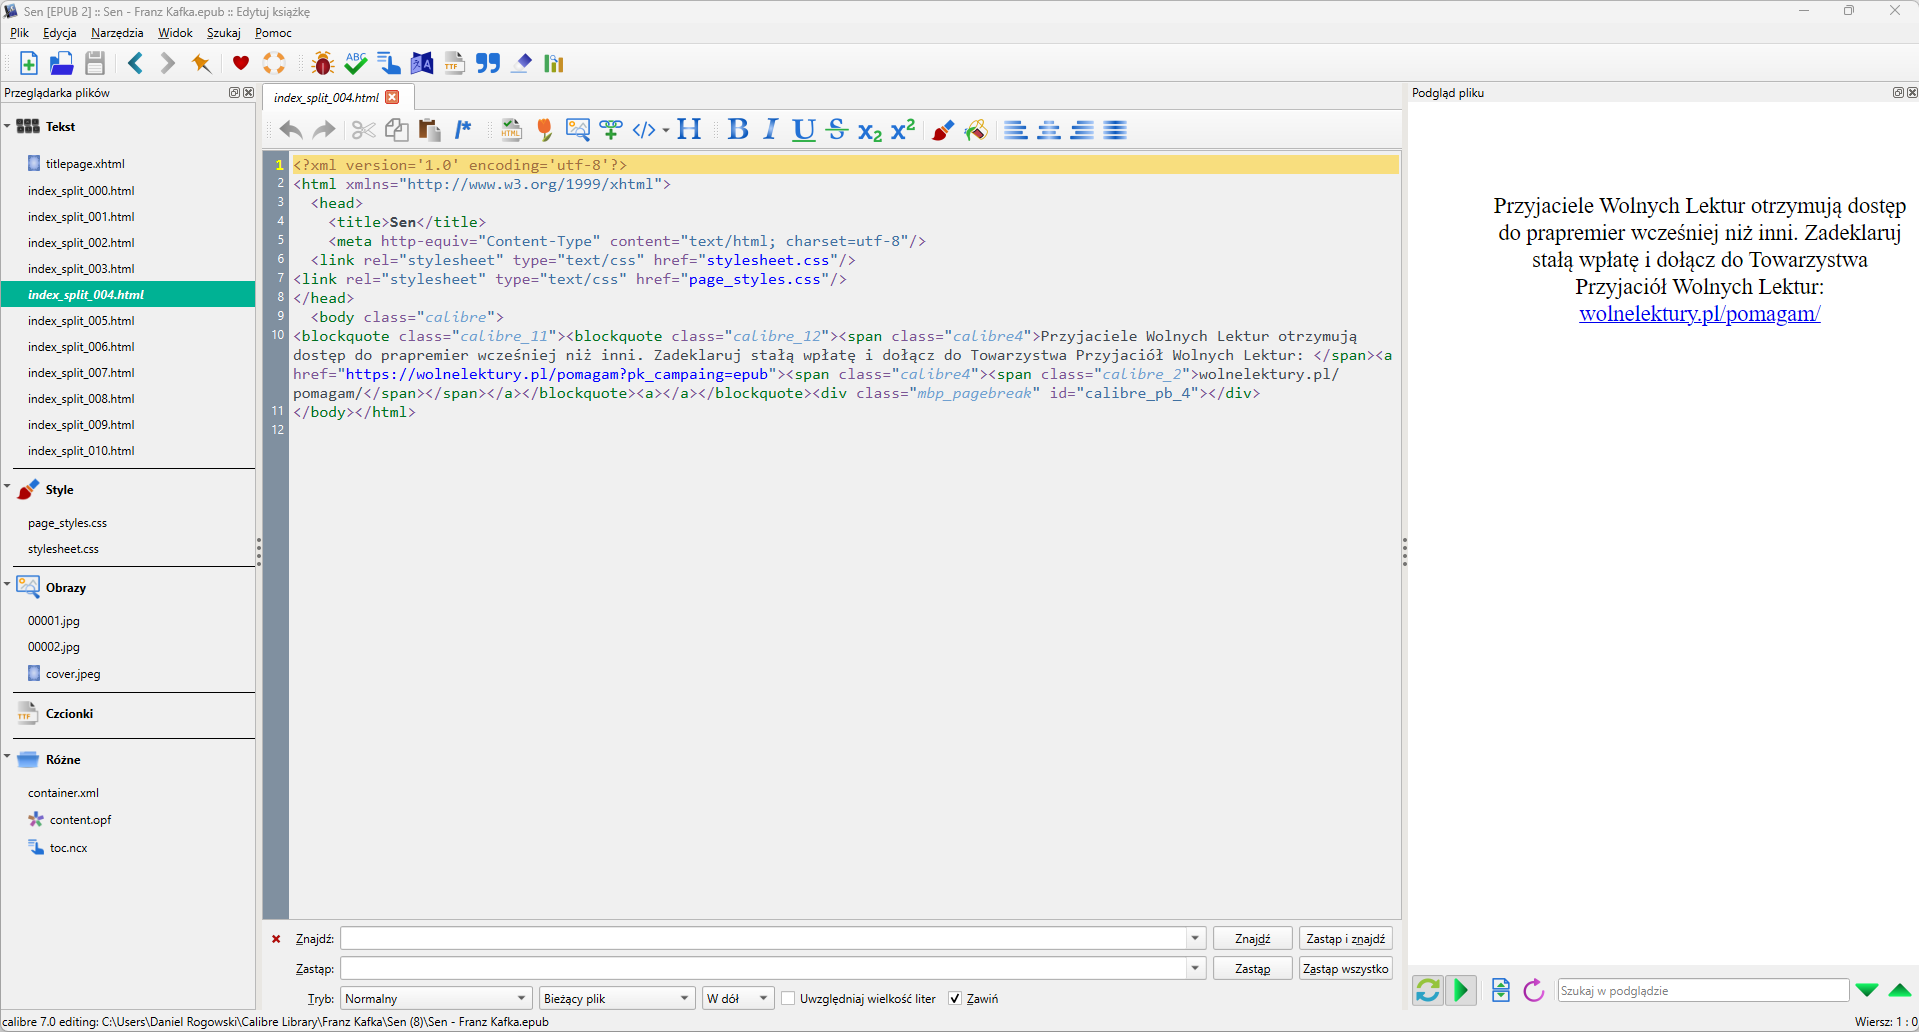
\includegraphics[width=0.9\textwidth]{chap2/calibre_editor.png}}
    \caption{Edytor e-booków programu Calibre}
    \label{fig:obrazek_z_ramką}
\end{figure}

Jedną z wad Calibre jest brak wersji na systemy mobilne (Android oraz iOS). Aplikacja Ebook-Wizard, dzięki temu, że jest aplikacją przeglądarkową, może być uruchamiana na każdym rodzaju urządzenia.

Inną wadą Calibre są ograniczone możliwości sieciowe, czyli brak łatwej synchronizacji e-booków pomiędzy urządzeniami. Projekt Calibre co prawda pozwala uruchomić własny prywatny serwer udostępniający kolekcję e-booków w sieci, natomiast działa to na zasadzie utworzenia serwera w sieci lokalnej. Ebook-Wizard oferuje darmową przestrzeń dyskową po założeniu konta w serwisie, dzięki czemu może być lepszą alternatywą dla użytkowników, którzy nie są zaznajomieni z technologiami informatycznymi.

Przewagą Calibre nad Ebook-Wizardem jest natomiast brak ograniczonej przestrzeni dyskowej. Calibre korzysta z dysku twardego użytkownika, więc ogranicza go wyłącznie rozmiar przestrzeni dyskowej na komputerze. Ebook-Wizard posiada limit w wysokości 500 MB, który przeciwdziała nadmiernemu obciążeniu serwera.

Kolejną z zalet Calibre jest wsparcie dla bardzo dużej liczby formatów. Ebook-Wizard posiada wsparcie dla rozszerzeń: mobi, epub, azw3, pdf, docx, txt oraz html. W przypadku Calibre, lista wspieranych rozszerzeń jest większa. Wspierane są na przykłąd formaty: zip, rtf (Rich Text Format) oraz htmlz (archiwum z plikami HTML)."

Calibre, oprócz klienta z graficznym interfejsem użytkownika, oferuje również szereg narzędzi terminalowych. Wspomniane narzędzia umożliwiają na przykład programowe wywołanie konwersji pliku. Niektóre z narzędzi dostarczanych przez projekt Calibre są wykorzystywane przez backend programu Ebook-Wizard, co zostanie dokładniej omówione w Rozdziale \ref{chapter:implementation}. 

\subsection{Aplikacja Sigil}

Aplikacja Sigil, w przeciwieństwie do Calibre, skupia się na aspekcie tworzenia e-booków.~\cite{sigil_user_guide} Podczas gdy głównym zadaniem Calibre jest przechowywanie i katalogowanie zbiorów, aplikacja Sigil jest dedykowana dla osób, które tworzą własnego e-booka od zera lub modyfikują istniejący plik.

Identycznie jak Calibre, Sigil również jest aplikacją z interfejsem graficznym, udostępnianą na otwartoźródłowej licencji GNU GPL 3. Ponadto, Sigil również nie uruchamia się na urządzeniach mobilnych, więc nad książką można pracować wyłącznie przy użyciu komputera. Twórcy programu Sigil udostępniają oficjalne instalatory dla systemów Windows oraz MacOS. Na stronie projektu Sigil widnieje informacja o tym, że projekt poprawnie kompiluje się również na Linuxie, aczkolwiek nie ma oficjalnego wsparcia dla tego systemu operacyjnego.

Sigil jest aplikacją dedykowaną dla formatu epub, nie ma możliwości zaimportowania e-booka w innym formacie. Przed edycją w programie Sigil, każdy e-book musi być przekonwertowany na format epub (na przykład programem takim jak Calibre).

Podobnie jak w przypadku Calibre, wadą tego edytora jest konieczność znajomości HTML oraz CSS, gdyż tworzenie e-booka opiera się na edytowaniu kodu źródłowego. 

\begin{figure}[h]
    \centering
    \setlength{\fboxsep}{0pt}
    \setlength{\fboxrule}{0.4pt}
    \fbox{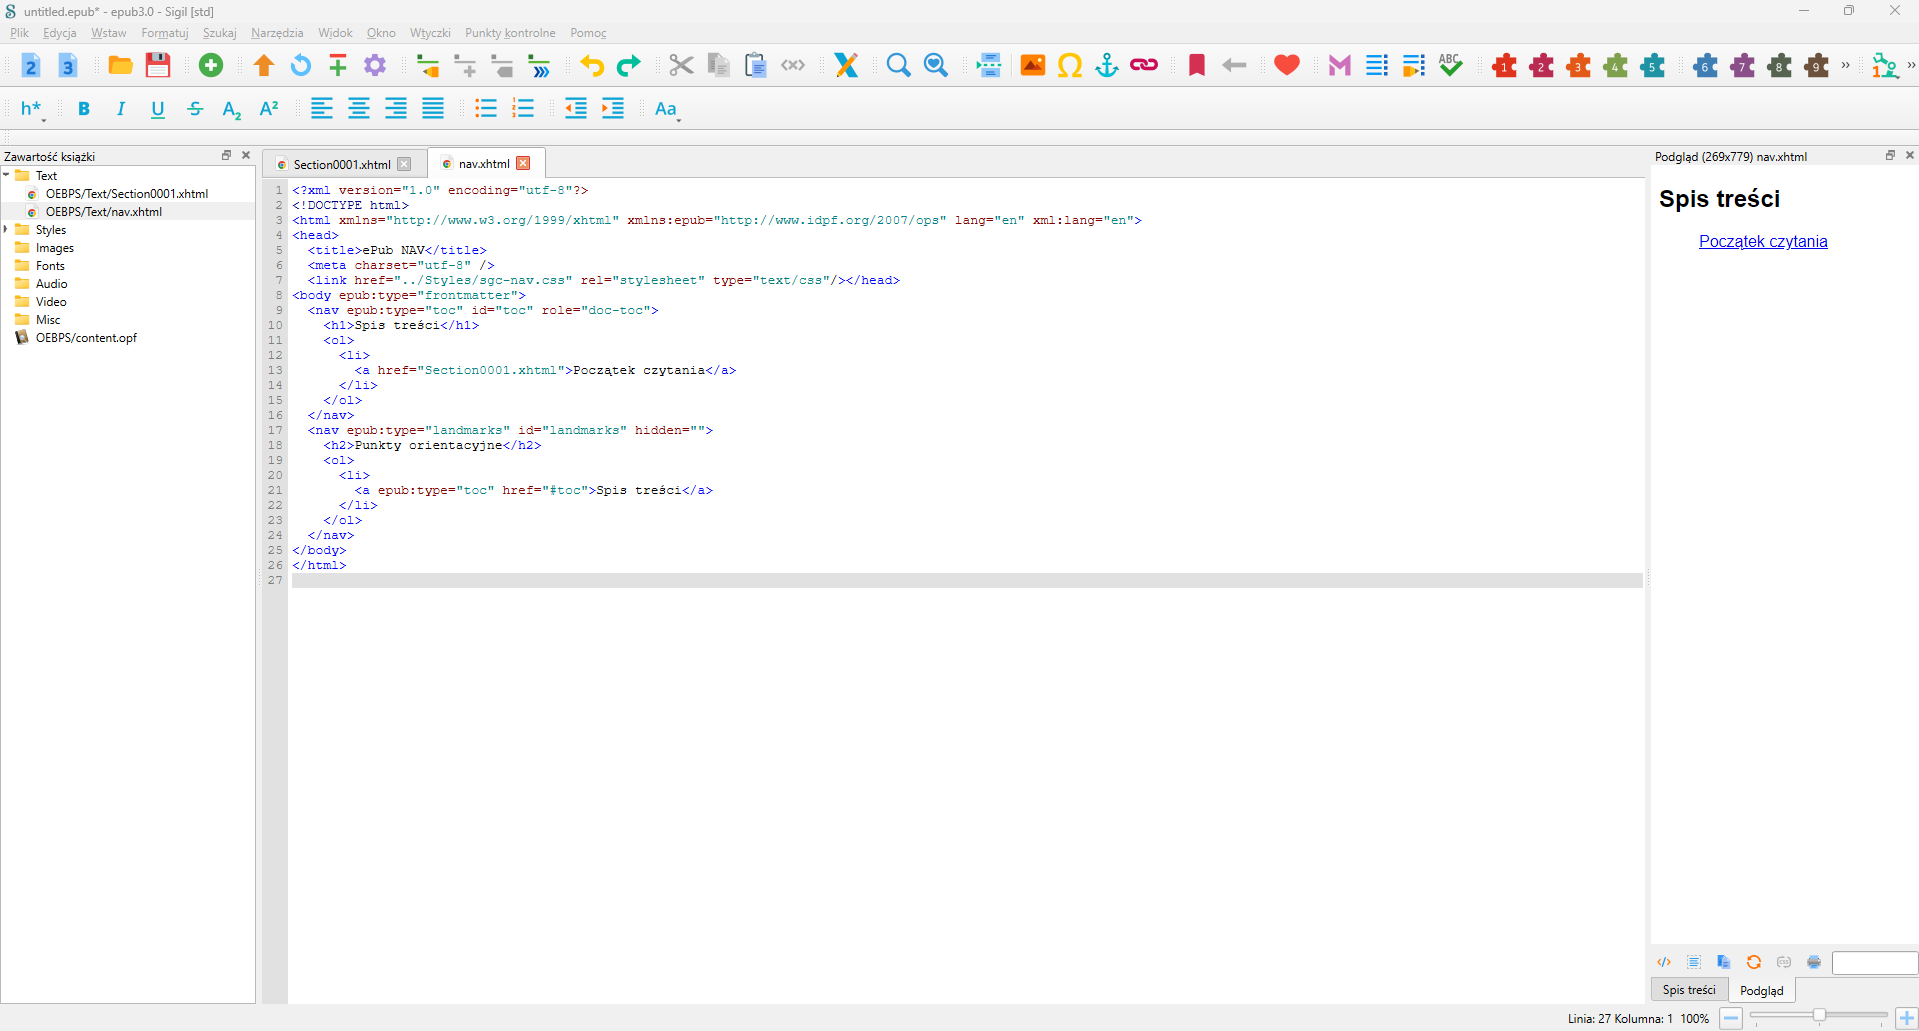
\includegraphics[width=0.9\textwidth]{chap2/sigil edytor.png}}
    \caption{Interfejs graficzny programu Sigil}
    \label{fig:obrazek_z_ramką}
\end{figure}

Aby zapewnić częściową możliwość edycji przy użyciu edytora WYSIWYG, autorzy programu Sigil przygotowali osobny program, PageEdit. Jest to graficzny edytor HTML, który pozwala na wizualną edycję dokumentów html wchodzących w skład pliku epub. \cite{sigil_user_guide}

Nie zastępuje to jednak pełnoprawnego edytora, jaki posiada na przykład Ebook-Wizard. Przy użyciu PageEdit co prawda można edytować pojedyncze pliki html wchodzące w skład pliku epub, natomiast dalej wymagana jest wiedza w zakresie budowy pliku epub (struktura katalogów, nazewnictwo plików, sposób osadzania metadanych). Ebook-Wizard ukrywa przed użytkownikiem te szczegóły i nie wymaga od niego żadnej technicznej wiedzy.

Sigil nie posiada też żadnych wbudowanych możliwości synchronizacji pracy pomiędzy urządzeniami. Jest to kolejna przewaga programu Ebook-Wizard, który pozwala na zapisanie pracy nad książką i kontynuowanie jej na innym urządzeniu.

\begin{figure}[h]
    \centering
    \setlength{\fboxsep}{0pt}
    \setlength{\fboxrule}{0.4pt}
    \fbox{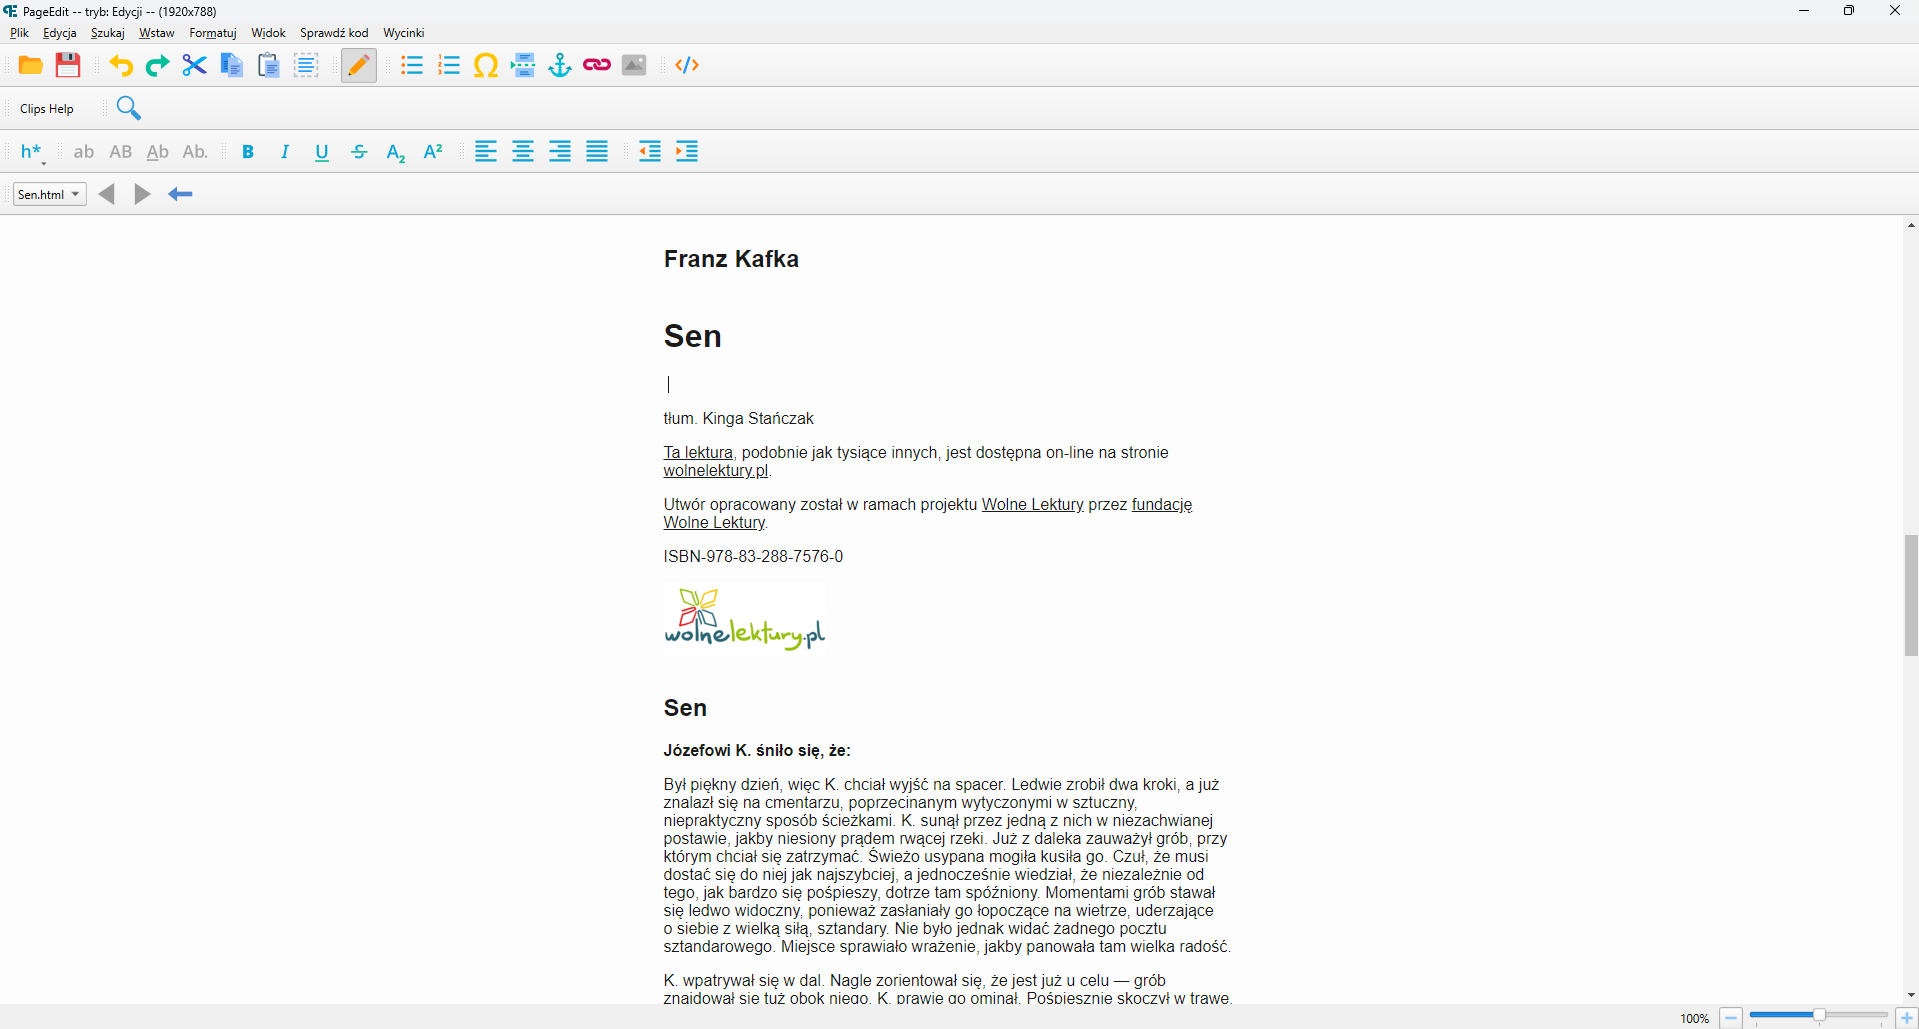
\includegraphics[width=0.9\textwidth]{chap2/pageedit.png}}
    \caption{Interfejs graficzny programu PageEdit}
    \label{fig:obrazek_z_ramką}
\end{figure}

\subsection{Aplikacja BookFusion}

BookFusion to aplikacja, której charakterystyka jest najbardziej zbliżona do funkcjonalności Ebook-Wizard. W przeciwieństwie do omawianych wcześniej programów Sigil i Calibre, BookFusion oferuje dostęp do e-booków z przeglądarki, udostępniając użytkownikom możliwość przechowywania e-booków na serwerze usługi. \cite{bookfusion_general_help_huide}

Dużą zaletą BookFusion jest integracja z darmowymi bibliotekami online. Korzystając z BookFusion, można w łatwy sposób zaimportować książkę z wybranych usług oferujących e-booki w domenie publicznej. BookFusion zawiera też sklep, w którym można zakupić książki wybranych wydawnictw.

BookFusion, w przeciwieństwie do wcześniej omawianych programów, jest aplikacją komercyjną. Darmowe konto pozwala na przechowywanie wyłącznie 10 e-booków, a liczbę tę można poszerzyć poprzez zakupienie płatnej subskrypcji. Dla porównania, Ebook-Wizard pozwala za darmo przechować dowolną liczbę e-booków, pod warunkiem, że przesłane pliki nie przekraczają limitu 500 MB. 

BookFusion nie udostępnia możliwości konwertowania e-booków pomiędzy formatami. Można zaimportować plik posiadający jedno ze wspieranych rozszerzeń, natomiast nie ma możliwości zmiany tego formatu już po przesłaniu pliku na serwer usługi.

BookFusion nie wspiera tworzenia e-booków, skupiając się wyłącznie na aspekcie gromadzenia i czytania. 

Podobnie jak Ebook-Wizard, BookFusion również oferuje możliwość przesłania książki na czytnik e-booków za pośrednictwem protokołu e-mailowego. Funkcja ta jest jednak ograniczona wyłącznie do adresów z domeny producenta Amazon Kindle. W aplikacji Ebook-Wizard takie ograniczenie nie występuje.

\begin{figure}[h]
    \centering
    \setlength{\fboxsep}{0pt}
    \setlength{\fboxrule}{0.4pt}
    \fbox{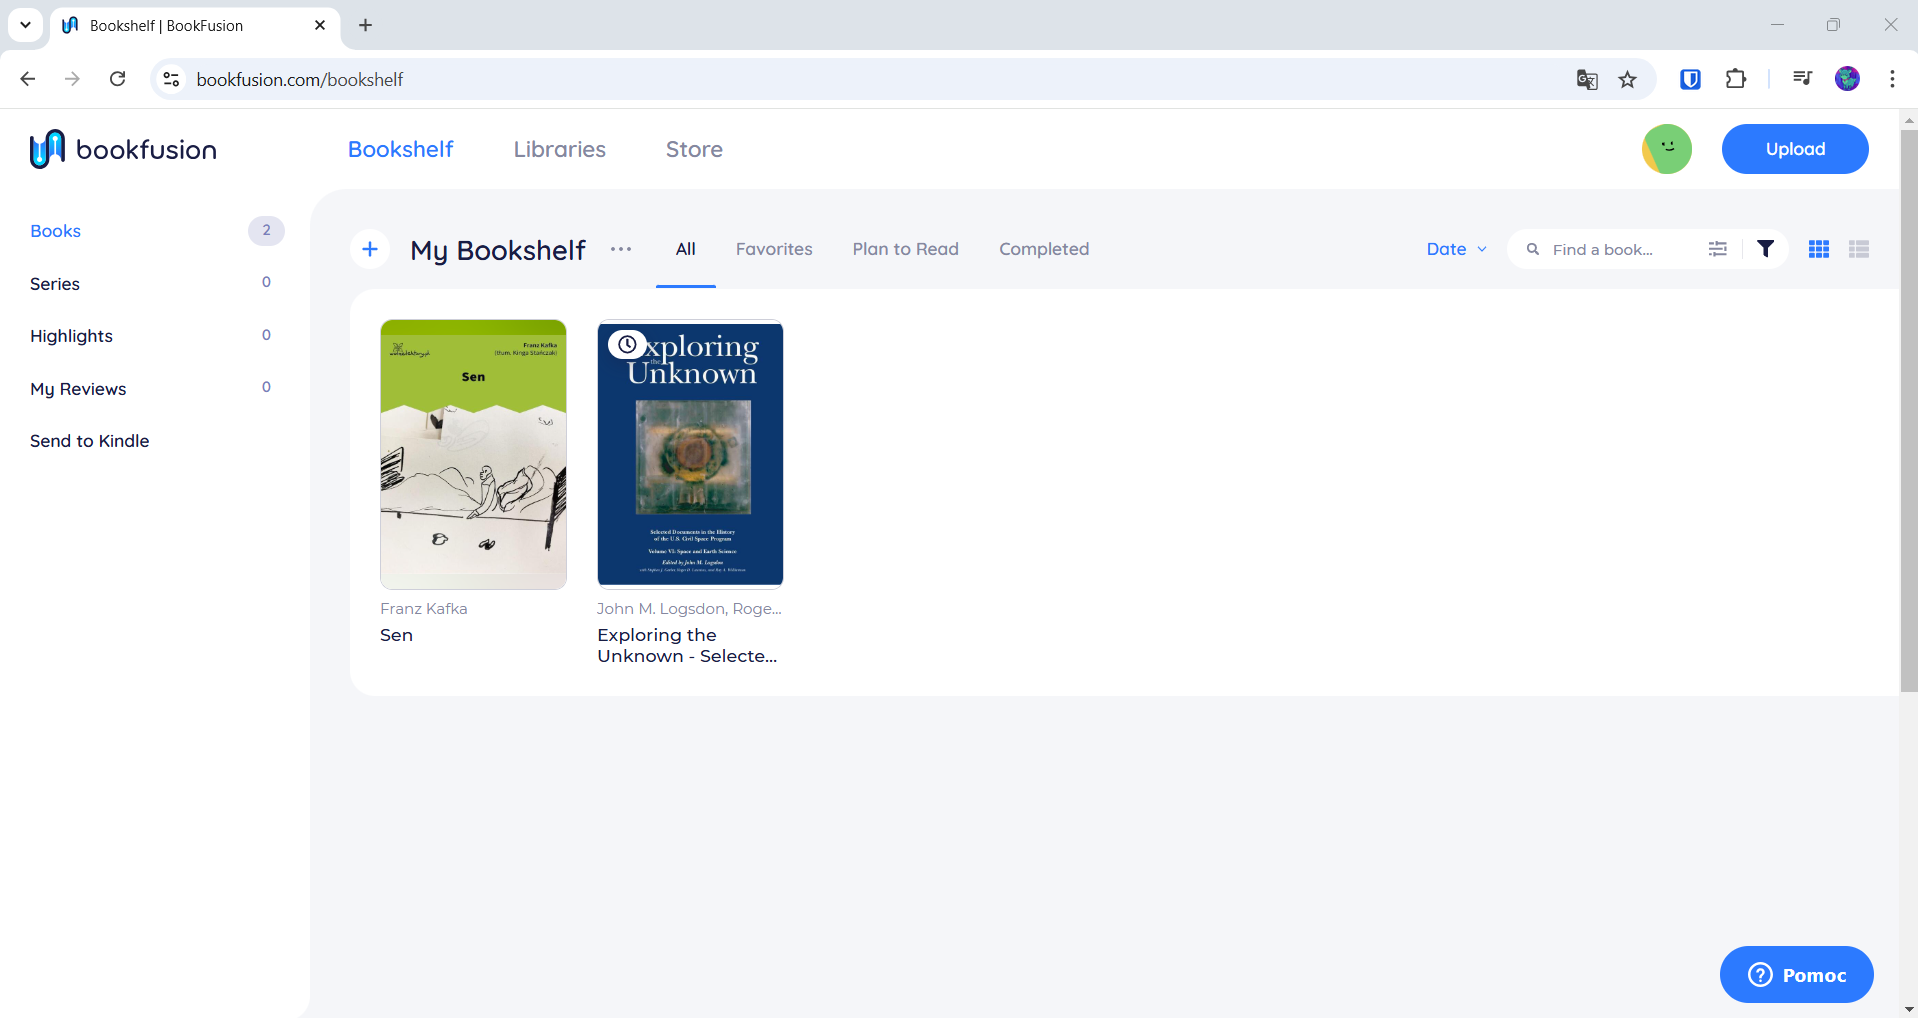
\includegraphics[width=0.9\textwidth]{chap2/page_book_fusion.png}}
    \caption{Interfejs graficzny programu EbookFusion}
    \label{fig:obrazek_z_ramką}
\end{figure}

\subsection{Tabelaryczne porównanie aplikacji}

W Tabeli \ref{tab:other_apps_comparision} przedstawiono wybrane funkcjonalności oferowane przez wspomniane aplikacje, zestawione z wybranymi funkcjonalnościami aplikacji Ebook-Wizard. Z zestawienia tablarycznego wynika, że większość funkcji oferowanych przez Ebook-Wizard można znaleźć również w rozwiązaniach konkurencyjnych. 

Wyjątkiem jest tutaj możliwość automatycznego wygenerowania audiobooka, która jest unikalna dla programu Ebook-Wizard. 

To, czym Ebook-Wizard wyróżnia się na rynku aplikacji e-bookowych, jest zebranie wszystkich istotnych funkcji oferowanych przez konkurencję i udostępnienie ich w formie pojedynczej aplikacji, dostępnej na każdym urządzeniu wyposażonym w przeglądarkę internetową.

Oznacza to, że Ebook-Wizard może zastąpić kilka różnych wyspecjalizowanych aplikacji, i udostępnić ich możliwości zarówno na komputerach, jak i tabletach, smartfonach i laptopach.

\begin{table}
    \renewcommand{\arraystretch}{1.5} % Ustawienie minimalnej wysokości rzędu
    \caption{Porównanie aplikacji konkurencyjnych do aplikacji Ebook-Wizard}

    \centering
    \begin{tabular}{|>{\centering\arraybackslash}m{4.7cm}|>{\centering\arraybackslash}m{2.7cm}|>{\centering\arraybackslash}m{2.1cm}|>{\centering\arraybackslash}m{2cm}|>{\centering\arraybackslash}m{2.3cm}|}
        \hline
        & \textbf{Ebook-Wizard} & \textbf{Calibre} & \textbf{Sigil}  & \textbf{Book-Fusion} \\ \hline
        Oferuje przechowywanie i katalogowanie e-booków & Tak & Tak & Nie & Tak \\ \hline
        Oferuje czytanie e-booków & Tak & Tak & Nie & Tak \\ \hline
        Oferuje tworzenie e-booków & Tak (WYSIWYG) & Tak (edycja kodu) & Tak (tylko epub) & Nie \\ \hline
        Umożliwia synchronizację e-booków & Tak & Tak (tylko własny serwer) & Nie & Tak \\ \hline
        Darmowy limit przechowywania & 500 MB, maks. 25 MB na plik & n/d & n/d & 10 plików \\ \hline
        Lektor SI (autom. generowanie audiobooka) & Tak & Nie & Nie & Nie \\ \hline
        Oferuje konwertowanie pomiędzy formatami & Tak & Tak & Nie & Nie \\ \hline
        Zawiera płatne subskrypcje & Nie & Nie & Nie & Tak \\ \hline
        Umożliwia przesłanie książki na czytnik & Tak & Tak (wymaga konfiguracji) & Nie & Tak (tylko Kindle) \\ \hline
        Środowisko uruchomieniowe & Przeglądarka & Komputer & Komputer & Przeglądarka \\
      \hline
    \end{tabular}
    \label{tab:other_apps_comparision}
\end{table}
